\documentclass[12pt]{article}
\setcounter{secnumdepth}{0}
\usepackage[english,greek]{babel}
\usepackage[utf8]{inputenc}
\usepackage{enumitem}
\usepackage{titling}
\usepackage{amsmath}
\usepackage{graphicx}
\usepackage{pgfplots}
\setlength{\droptitle}{-12em}
\usepackage{listings}
\lstset{
  basicstyle=\ttfamily,
  mathescape
}

\title{{Ανάλυση Σχεδίαση Συστημάτων Λογισμικού} \\
\vspace{2cm}
{\Huge Εργασία 2017-2018} \\
\vspace{2cm}
{Νέμανια Νέντις}\\
{Α.Μ. 111520140124}\\
{Κωνσταντίνος Στεφανίδης - Βοζίκης}\\
{Α.Μ. 1115201400192}}


\date{}

\begin{document}
\maketitle
\newpage
\tableofcontents
\newpage

\section{Διαδικαστικά}
Η εργασία αναπτύχθηκε από ομάδα 2 ατόμων. Η δουλειά μοιράστηκε ως εξής: 
Το πρώτο μέλος ασχολήθηκε κυρίως με τα μέρη Β και Γ καθώς και με το τελευταίο 
ερώτημα του μέρους Α. Το άλλο μέλος ασχολήθηκε κυρίως με τα ερωτήματα 1 εως 8 
του μέρους Α. Κάθε μέλος συμμετείχε στην συζήτηση για την διεκπαιρέωση 
όλων των μερών καθώς και στην επαλήθευση της ορθότητάς τους. Η συνεργασία έγινε 
με συναντήσεις αλλά και εξ αποστάσεως μέσω \textlatin{Skype}.

\newpage
\section{Αντικειμενοστραφής Ανάλυση και Σχεδιασμός}
\begin{enumerate}
\item
Οι μη λειτουργικές απαιτήσεις του συστήματος είναι:
\begin{itemize}
\item
Λήψη αντιγράφων (\textlatin{back up}) κάθε ώρα
\item
Λειτουργία του συστήματος 24 ώρες το 24ώρο
\end{itemize}
\item
\begin{tabular}{|l|l|}
\hline
'Εννοια & Περιγραφή \\
\hline
Διδάσκων & Υπάλληλος του πανεπιστημίου που διδάσκει \\
\hline
ΕΔΙΠ & Διδάσκων πλήρους απασχόλησης \\
\hline
Συμβασιούχος & Διδάσκων με σύμβαση συγκεκριμένου χρόνου \\
\hline
Συμβόλαιο & Συμφωνία μεταξύ του πανεπιστημίου και ενός συμβασιούχου \\
\hline
Άδεια & Χρονικό διάστημα που ένας μόνιμος διδάσκων δεν δουλέυει \\ 
\hline
Τρόπος πληρωμής & Τρόπος με τον οποίο ένας διδάσκων λαμβάνει την αμοιβή \\ 
& του από το πανεπιστήμιο \\
\hline
Ειδοποίηση πληρωμής & Τρόπος με τον οποίο ένας συμβασιούχος ενημερώνεται για \\
 & τα χρήματα που εισπράττει από το πανεπιστήμιο \\
\hline
Πληρωμή & Αμοιβή του πανεπιστημίου προς έναν διδάσκοντα για \\ 
& την εργασία του \\ 
\hline
Χρονοκάρτα & Κατάσταση στην οποία ένας συμβασιούχος διδάσκων \\
 & υποβάλλει στο σύστημα για να μετρηθούν οι μέρες \\
 &  και ώρες διδασκαλίας του. \\
\hline
\end{tabular}

\newpage
\item
Το διάγραμμα περιπτώσεων χρήσης είναι το παρακάτω:
\begin{center}
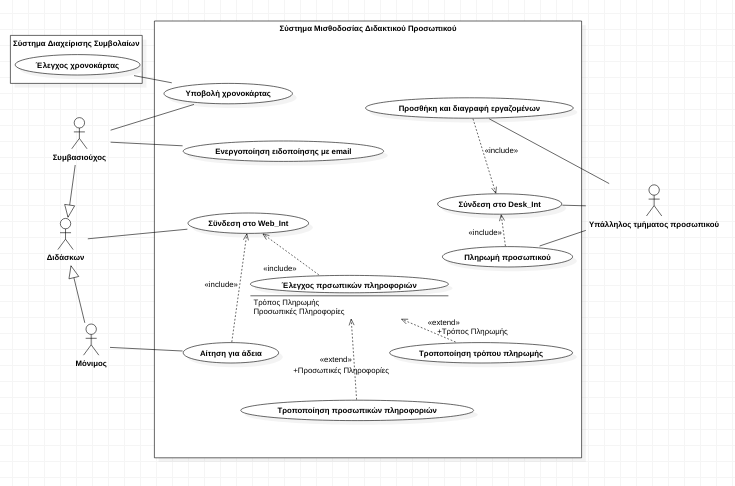
\includegraphics[scale=0.6]{use_case}
\end{center}

\newpage
\item
Το διάγραμμα κλάσεων είναι το παρακάτω:
\begin{center}
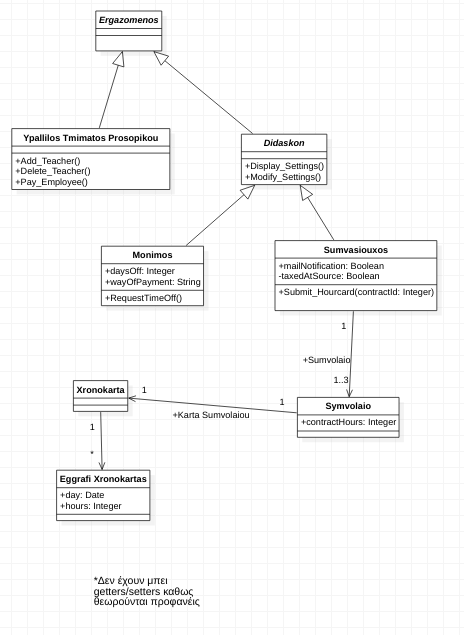
\includegraphics[scale=0.8]{class_diag}
\end{center}

\newpage
\item
\subsection*{Κύριο σενάριο επιτυχίας}
\begin{enumerate}[label=\arabic*.]
\item
Ο χρήστης ανοίγει το \textlatin{Web\_Int}
\item
Ο χρήστης δίνει τα στοιχεία για να κάνει \textlatin{login}
\item
To σύστημα επιβεβαιώνει τα στοιχεία του χρήστη.
\item
To σύστημα εμφανίζει την αρχική σελίδα του \textlatin{Web\_Int} στον χρήστη.
\item
Ο χρήστης διαλέγει την επιλογή "Τροποποίηση τρόπου πληρωμής" 
από το \textlatin{Web\_Int}.
\item
Το σύστημα εμφανίζει την σελίδα με τις επιλογές για τον τρόπο 
πληρωμής στην χρήστη.
\item
Ο χρήστης διαλέγει τον εναλλακτικό τρόπο πληρωμής που επιθυμεί.
\item
Το σύστημα εμφανίζει μήνυμα επιτυχίας αλλαγής τρόπου πληρωμής 
στον χρήστη.
\item
Ο χρήστης κάνει \textlatin{logout} από το σύστημα.
\end{enumerate}

\subsection*{Επεκτάσεις}
3α το σύστημα δεν επιβεβαινει τα στοιχεία.
\begin{enumerate}[label=\arabic*.]
\item
Το σύστημα εμφανίζει μήνυμα λάθους και ζητά από τον 
χρήστη να ξαναεισάγει τα στοιχεία του.
\item 
Ο χρήστης πληκτρολογεί ξανά τα στοιχεία του.
\end{enumerate}

\newpage
\item
Το διάγραμμα δραστηριοτήτων για τη διαδικασία χορήγηση άδειας είναι το παρακάτω:
\begin{center}
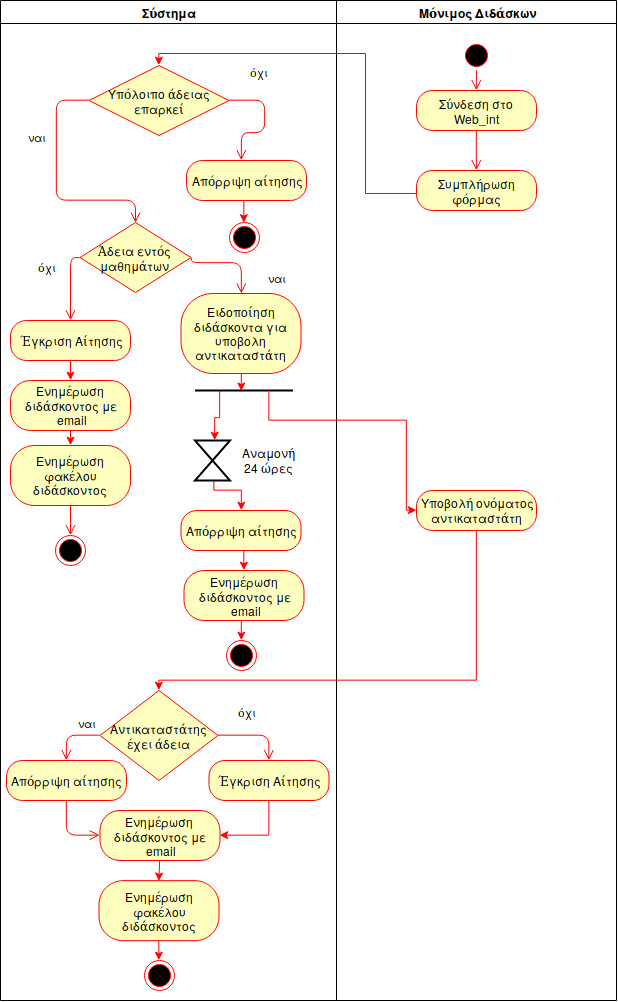
\includegraphics[scale=0.5]{activity}
\end{center}

\newpage
\item
Το διάγραμμα καταστάσεων για το αντικείμενο «Αίτηση Άδειας» είναι το παρακάτω:
\begin{center}
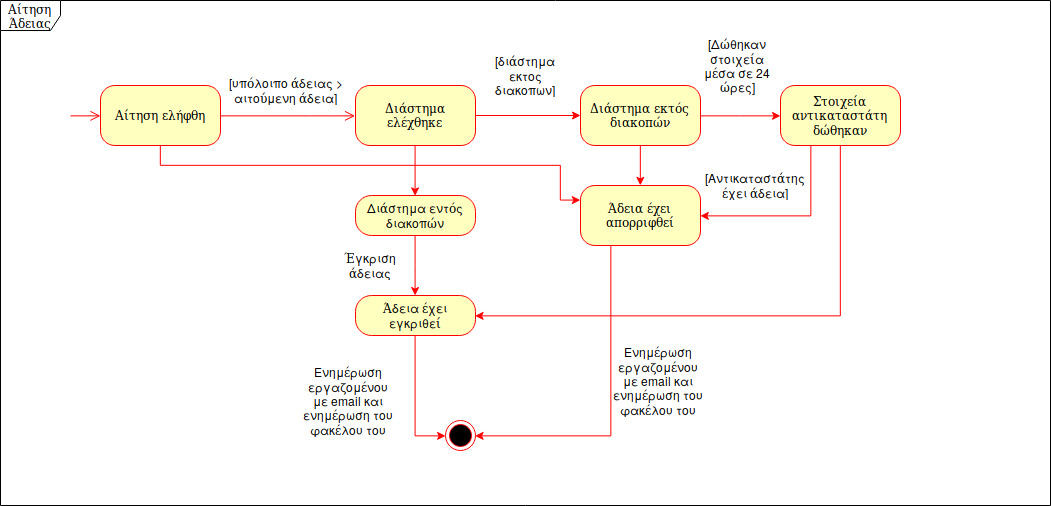
\includegraphics[scale=0.35]{state_diag}
\end{center}

\item
Το διάγραμμα ακολουθίας για την διαδικασία πληρωμής είναι το παρακάτω:
\begin{center}
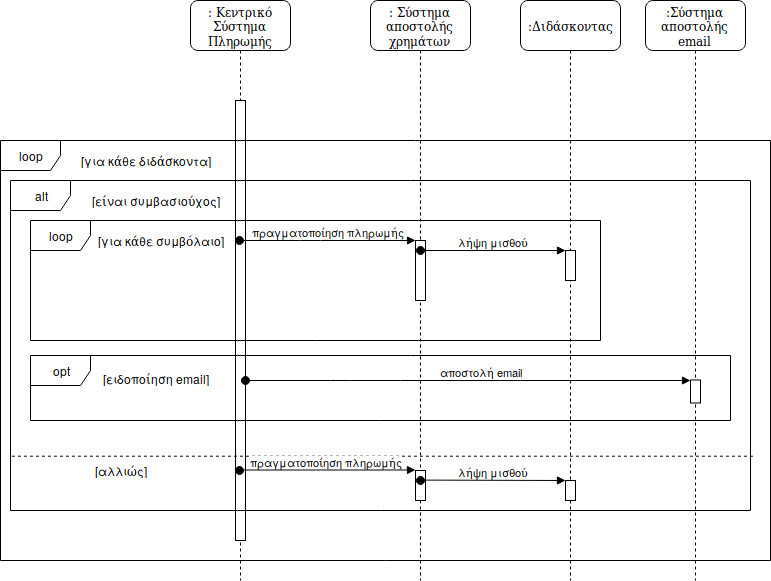
\includegraphics[scale=0.45]{sequence}
\end{center}

\newpage
\item
\end{enumerate}


\section{Δομημένη Ανάλυση}

\begin{center}
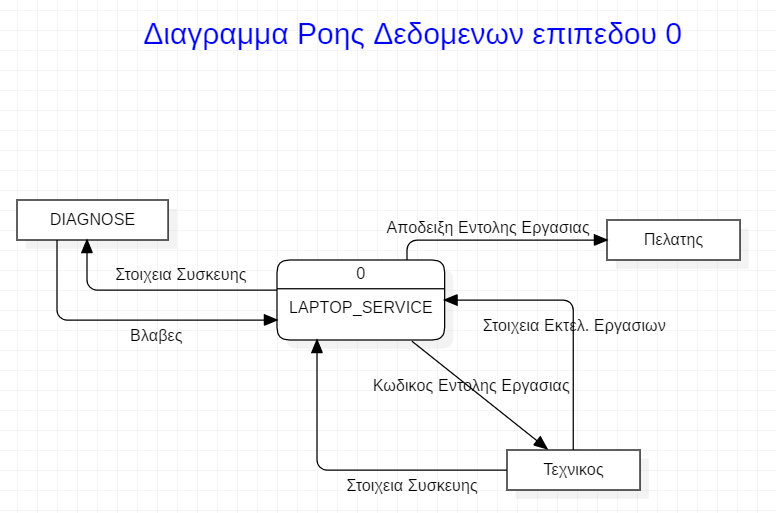
\includegraphics[scale=1]{MerosB/B1}
\end{center}
\begin{center}
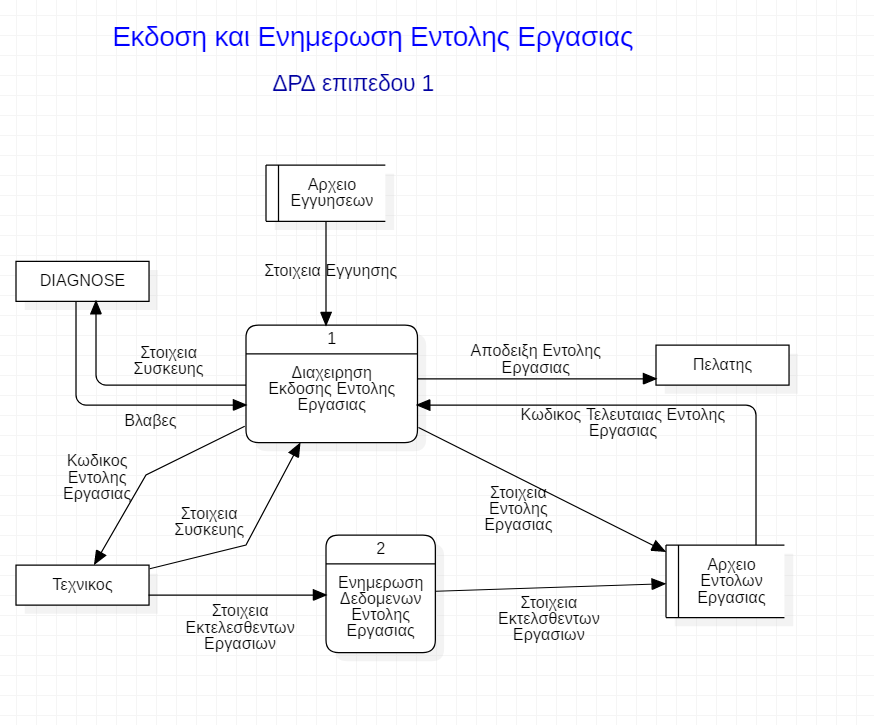
\includegraphics[scale=1]{MerosB/B2}
\end{center}
\begin{center}
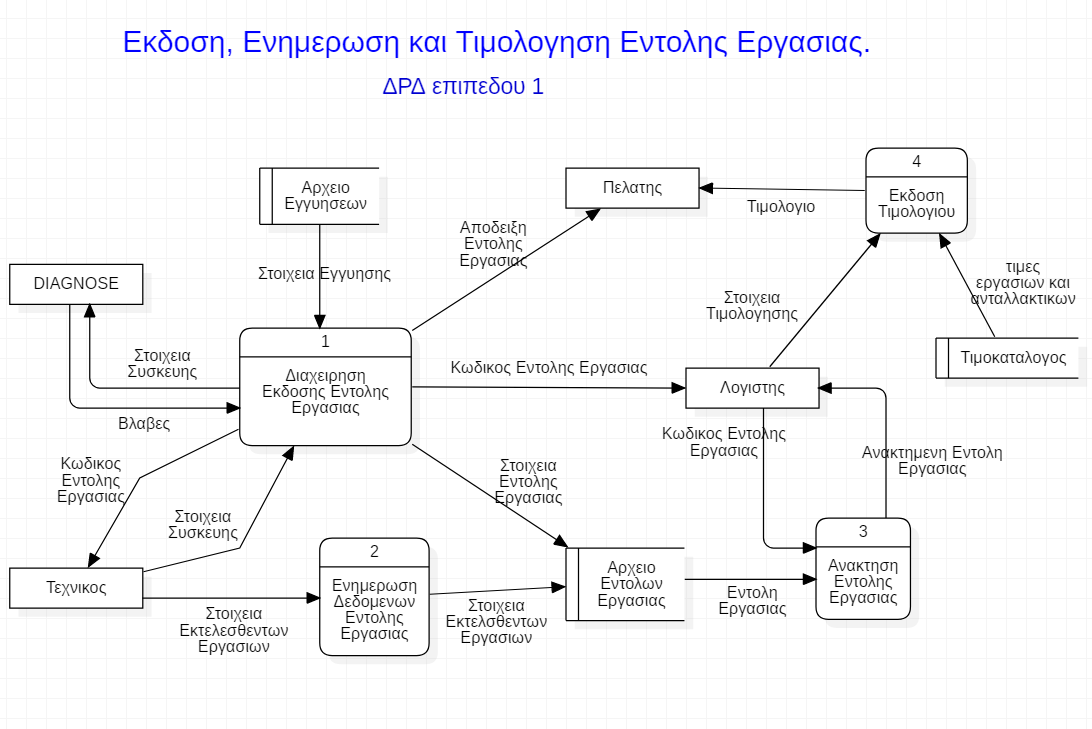
\includegraphics[scale=0.7]{MerosB/B3}
\end{center}
\begin{center}
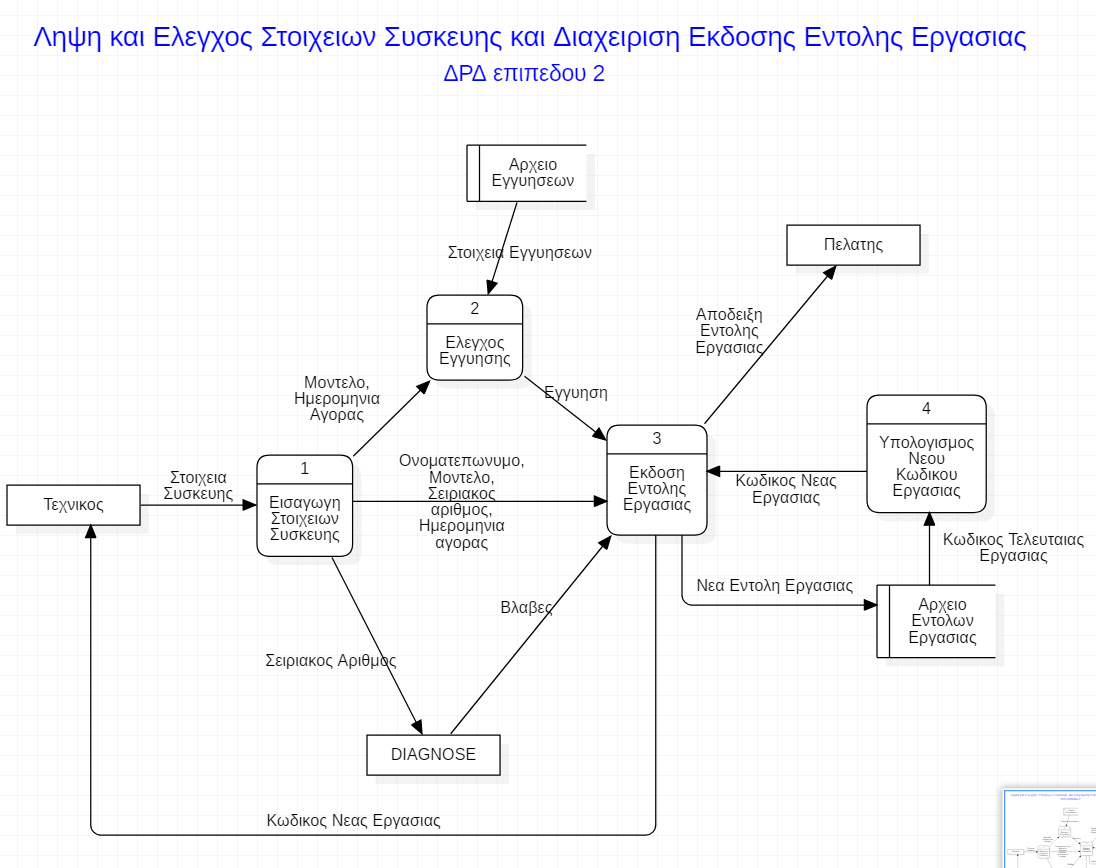
\includegraphics[scale=0.7]{MerosB/B4}
\end{center}
Παρατηρησεις: Με επιφυλαξη η ροη προς $DIAGNOSE$ απο την εφαρμογη καθως δεν διευκρινιζεται απο την εκφωνηση η χρησιμοτητα του.
\newpage
\section{Δομημένος Σχεδιασμός}
\begin{enumerate}

\item Ως κεντρικό μετασχηματισμό επιλέγουμε τον $P1$, καθώς ο $P1$ 
δέχεται δεδομένα εισόδου και εκείνος επενεργεί σε αυτά προκειμένου να δημιουργηθούν δεδομένα εξόδου.\\
Παρατηρηση: Αν θελαμε να επιλεξουμε Κεντρο Δοσοληψιων ο καταλληλος μετασχηματισμος θα ηταν ο $P3$.

\begin{center}
\begin{tabular}{c}
Το Διάγραμμα Δομάς Προγράμματος (ΔΔΠ) ειναι:\\
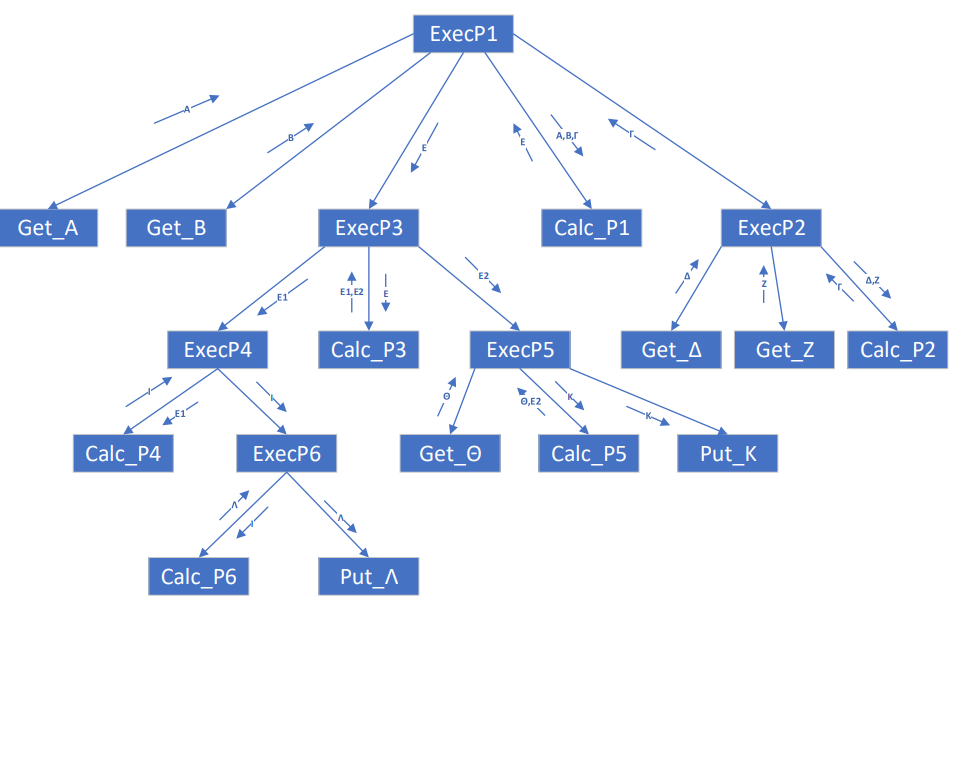
\includegraphics[scale=0.5]{MerosG/DDP}
\end{tabular}
\end{center}

\newpage
\item Τμηματα Ψευδοκωδικα:
\begin{enumerate}[label*=\roman*]
	\item Mονάδα ελέγχου του μετασχηματισμού Ρ1
	
	\begin{lstlisting}
	$Procedure$ $ExecP1$
		$Local$ $var$ A,B,G,E
		$Arxikopoihse$ A,B,G,E
		$Call$ $Get\_A(A)$
		$Call$ $Get\_B(B)$
		$Call$ $Calc\_P1($A,B,G,E$)$
		$Call$ $ExecP3(E)$
	$End\_Procedure$
	\end{lstlisting}
	
	\item  Μονάδα υπολογισμού του μετασχηματισμού Ρ2
	\begin{lstlisting}
	$Procedure$ $Calc\_P2($D$,$Z$:IN,$G$:IN/OUT)$
		...
		$Upologise$ G
		...
	$End\_Procedure$
	\end{lstlisting}
	
	\item Μονάδα παρουσίασης του μετασχηματισμού Ρ5
	\begin{lstlisting}
	$Procedure$ $Put\_K(K:IN)$
		...
		$Grapse$ K
		...
	$End\_Procedure$
	\end{lstlisting}
	
	\item Μονάδα διαχείρισης δεδομένων του μετασχηματισμού Ρ1
	\begin{lstlisting}
	$Procedure$ $Get\_B(B:IN/OUT)$
		...
		$Diavase$ B
		...
	$End\_Procedure$
	\end{lstlisting}
\end{enumerate}
\end{enumerate}

\end{document}